% mechanism: a box whose declared size is stored as a String attribute (diagbox, rotate.sty's `\rotate[f|u]`,
%          makecell's `\diaghead`) gives its foreignObject the measured size: the String is no Dimension.
% witness: synthetic (revDTL1a B1; 0 of 21 census diagbox+tikz papers have such a node)
% oracle:  pdflatex 0 errors; boxes 1 33.1112pt x 14.5pt + 9.5pt, 2 29.7223pt x 6.94444pt + 1.94444pt
% engines: perl 0 errors: 1 29.22x19.22, 2 7.69x109.24; rust int160b: 1 28.44x9.61, 2 41.51x12.3; DTL1a: both 0x0
%          (the String read as 0)
% expect:  0 errors; int160b's two measured sizes
% status:  RED -> GREEN (DTL1b, guard perfect_kernel_batch56::a_node_takes_its_boxs_declared_size)
\documentclass{article}
\usepackage{tikz,diagbox,rotate}
\begin{document}
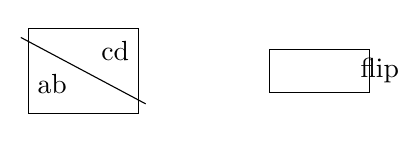
\begin{tikzpicture}
\node[draw] at (0,0) {\diagbox{ab}{cd}};
\node[draw] at (3,0) {\rotate[f]{flipped}};
\end{tikzpicture}
\end{document}
